\documentclass{standalone}
\usepackage{tikz}
\usetikzlibrary{positioning,matrix,backgrounds}
\begin{document}

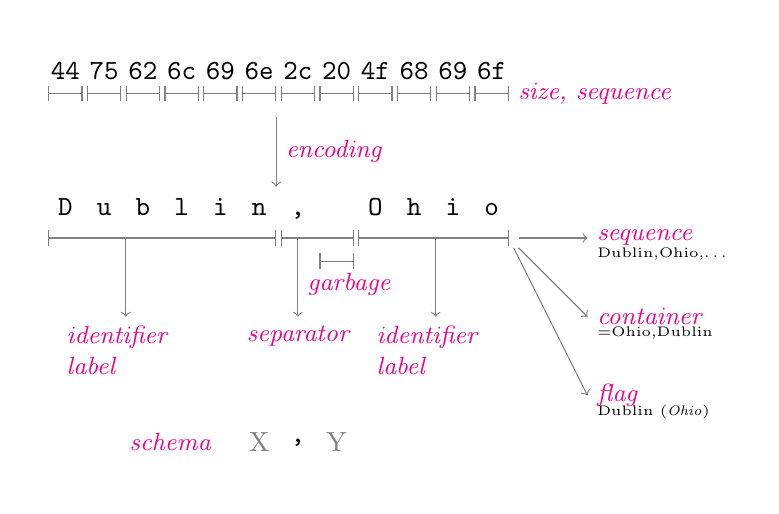
\begin{tikzpicture}[
    pattern/.style={font=\itshape\small,text=magenta},
    show background rectangle,background rectangle/.style={fill=white}
]

\matrix[matrix of nodes,column sep=2pt,
    nodes={font=\ttfamily,text width=1.2em,minimum height=3.8ex,inner sep=0,align=center}] (s) {
  44 & 75 & 62 & 6c & 69 & 6e & 2c & 20 & 4f & 68 & 69 & 6f \\
  ~ & ~ & ~ & ~ & ~ & ~ & ~ & ~ & ~ & ~ & ~ & ~ \\
  ~ & ~ & ~ & ~ & ~ & ~ & ~ & ~ & ~ & ~ & ~ & ~ \\
  D & u & b & l & i & n & , & ~ & O & h & i & o \\
  ~ & ~ & ~ & ~ & ~ & ~ & ~ & ~ & ~ & ~ & ~ & ~ \\
  ~ & ~ & ~ & ~ & ~ & ~ & ~ & ~ & ~ & ~ & ~ & ~ \\
  ~ & ~ & ~ & ~ & ~ & ~ & ~ & ~ & ~ & ~ & ~ & ~ \\
  ~ & ~ & ~ & ~ & ~ & ~ & ~ & ~ & ~ & ~ & ~ & ~ \\
  ~ & ~ & ~ & ~ & ~ & ~ & , & ~ & ~ & ~ & ~ & ~ \\
};

\draw (s-9-6) node[gray] {X};
\draw (s-9-8) node[gray] {Y};
\draw (s-9-5) node[anchor=east,pattern] {schema};

\foreach \n in {1,...,12}{
  \draw[|-|,gray] (s-2-\n.north west) to (s-2-\n.north east);
}

\draw[|-|,gray] (s-5-1.north west) to (s-5-6.north east);
\draw[|-|,gray] (s-5-7.north west) to (s-5-8.north east);
\draw[|-|,gray] (s-5-9.north west) to (s-5-12.north east);
\draw[|-|,gray] (s-5-8.west) to (s-5-8.east);

\draw[->,gray] (s-2-6.east) to 
    node[anchor=west,pattern] {encoding}
(s-4-6.north east);

\draw[gray,->] (s-5-7.north) to ++(0,-1cm)
    node[pattern,anchor=north] (g) {separator};
\draw[gray,->] (s-5-3.north west) to ++(0,-1cm)
  node [text width=1.5cm,pattern,anchor=north] {identifier\\label};
\draw[gray,->] (s-5-11.north west) to ++(0,-1cm)
   node [text width=1.5cm,pattern,anchor=north] {identifier\\label};

\node[pattern,below=0ex of s-5-7.south,anchor=west] {garbage};

\node[pattern,right=0 of s-2-12.north east] {size, sequence};
\draw (s-5-12.north east) node (x) {};

\draw[gray,->] (x) to ++(1cm,0mm) node (a) {};
\draw[gray,->] (x) to ++(1cm,-1cm) node (b) {};
\draw[gray,->] (x) to ++(1cm,-2cm) node (c) {};

\draw (a) node [anchor=west,pattern] {sequence}
          node [anchor=north west,font=\tiny] {Dublin,Ohio,\ldots};
\draw (b) node [anchor=west,pattern] {container}
          node [anchor=north west,font=\tiny] {=Ohio,Dublin};
\draw (c) node [anchor=west,pattern] {flag}
          node [anchor=north west,font=\tiny] {Dublin (\textit{Ohio})};

\end{tikzpicture}
\end{document}
